\section{Konzept}

In diesem Kapitel wird das Konzept beschrieben, wie man eine Last Lokalisieren kann mit Marker.
Als erstes werden die Anforderungen angeschaut, welche das System erfüllen muss. 
Danach wird die Lokalisierung mit Marker beschrieben, sowie welche Eigenschaften die Marker haben müssen.
Weiters werden die mindest Kamera Eigenschaften aufgezählt und berechnet.
Zum Schluss wird das Konzept evaluiert.

\subsection{Überblick}
Ludwig Systems benötigt eine Lösung, welche von der Traverse aus die Ist-Koordinaten, die Rotation und Neigung der Last ausgibt. Das Konzept soll dieses Ziel erfüllen um in der Zukunft die Traverse automatisch bewegen zu können. Des Weiteren soll das Konzept sicherstellen, dass die Genauigkeiten ,welche vom Kunden gegeben wurde, eingehalten werden können. 
Da sich die Art von Last ändern kann, wurde der Fokus auf die Lokalisierung der Anschlagspunkte gelegt. 
Es wurden 2 Konzepte ausgearbeitet, welche diese Ziele erfüllen können. Beim ersten Konzept wird ein Machine-Learning Modell benutzt um die Anschlagspunkte zu erkennen und 3D Lokalisierung durchzuführen und beim zweiten Konzept werden die Anschlagspunkte durch AR Marker 
Lokalisiert.

\subsection{Anforderungen}\label{requirements}

Folgende Anforderungen muss das System erfüllen:

\begin{center}
    \begin{tabular}{ |l|l| }
        \hline
        \textbf{Anforderung} & \textbf{Beschreibung} \\ \hline
        X/Y Genauigkeit & Ungenauigkeit: ±2 cm \\ \hline
        Z Genauigkeit & Ungenauigkeit: ±1 cm \\ \hline
        Rotation & Ungenauigkeit: ±2° \\ \hline
        Neigung & Ungenauigkeit: ±1° \\ \hline
        Kamera Kalibrierung & Kalibrierung und Speicherung möglich \\ \hline
        Anschlagspunkte & Ausgabe der Koordinaten \\ \hline
    \end{tabular}
    \end{center}


\subsection{Konzept: Lokalisierung durch AR Marker}

In diesem Konzept geht es darum die Anschlagspunkte durch AR Marker, wie ArUco oder AprilTags, zu lokalisieren. Dabei werden die Marker um den Anschlagspunkt angeordnet. Wenn die Marker dann erkannt werden, kann durch Posenschätzung die 3D Koordinaten und 3D Rotationen berechnet werden. Durch die Anordnung der Marker kann dann die 3D Koordinaten vom Anschlagspunkt berechnet werden. 
Für dieses Konzept werden Sticker von den Markern benötigt, welche eine genaue Grösse haben. 

\subsubsection{Marker Anordnung}

Wie in der Abbildung (ref) zu sehen ist werden 4 Marker in einem Kreuz-Muster um den Anschlagspunkt angeordnet. Für Anschlagspunkt 1 werden Marker mit den IDs von 0 bis 3 benutzt und in der Reihenfolge links, oben, rechts und dann unten angeordnet. Für Anschlagspunkt 2 Marker mit den IDs von 4 bis 7 benutzt. Dadurch können zwischen den zwei Anschlagspunkten differenziert werden wenn beide Anschlagspunkte im Bild sind.Falls weitere Anschlagspunkte benötigt werden, sollten die Marker-IDs-Reihenfolge und Position fortgeführt werden. Diese Anordnung sorgt dafür dass mindestens ein Marker erkannt werden kann, soweit die Traverse in der definierten Grenze ist. 
(redundanz erhöht stabilität)

\clearpage
\subsubsection{Markergrösse}

Die Markergrösse spielt eine zentrale Rolle, um die Anschlagspunkte präzise zu lokalisieren und 
die Berechnungen für die Ausrichtung der Traverse zuverlässig durchzuführen. Ein möglichst grosser 
Marker erhöht die Genauigkeit der Distanzberechnung und trägt damit zur Effizienz des Systems bei. 
Abbildung \ref{fig:marker} illustriert, wie die optimale Markergrösse in Abhängigkeit vom gegebenen 
Radius \( R \) berechnet werden kann.

\begin{figure}[H]
    \centering
    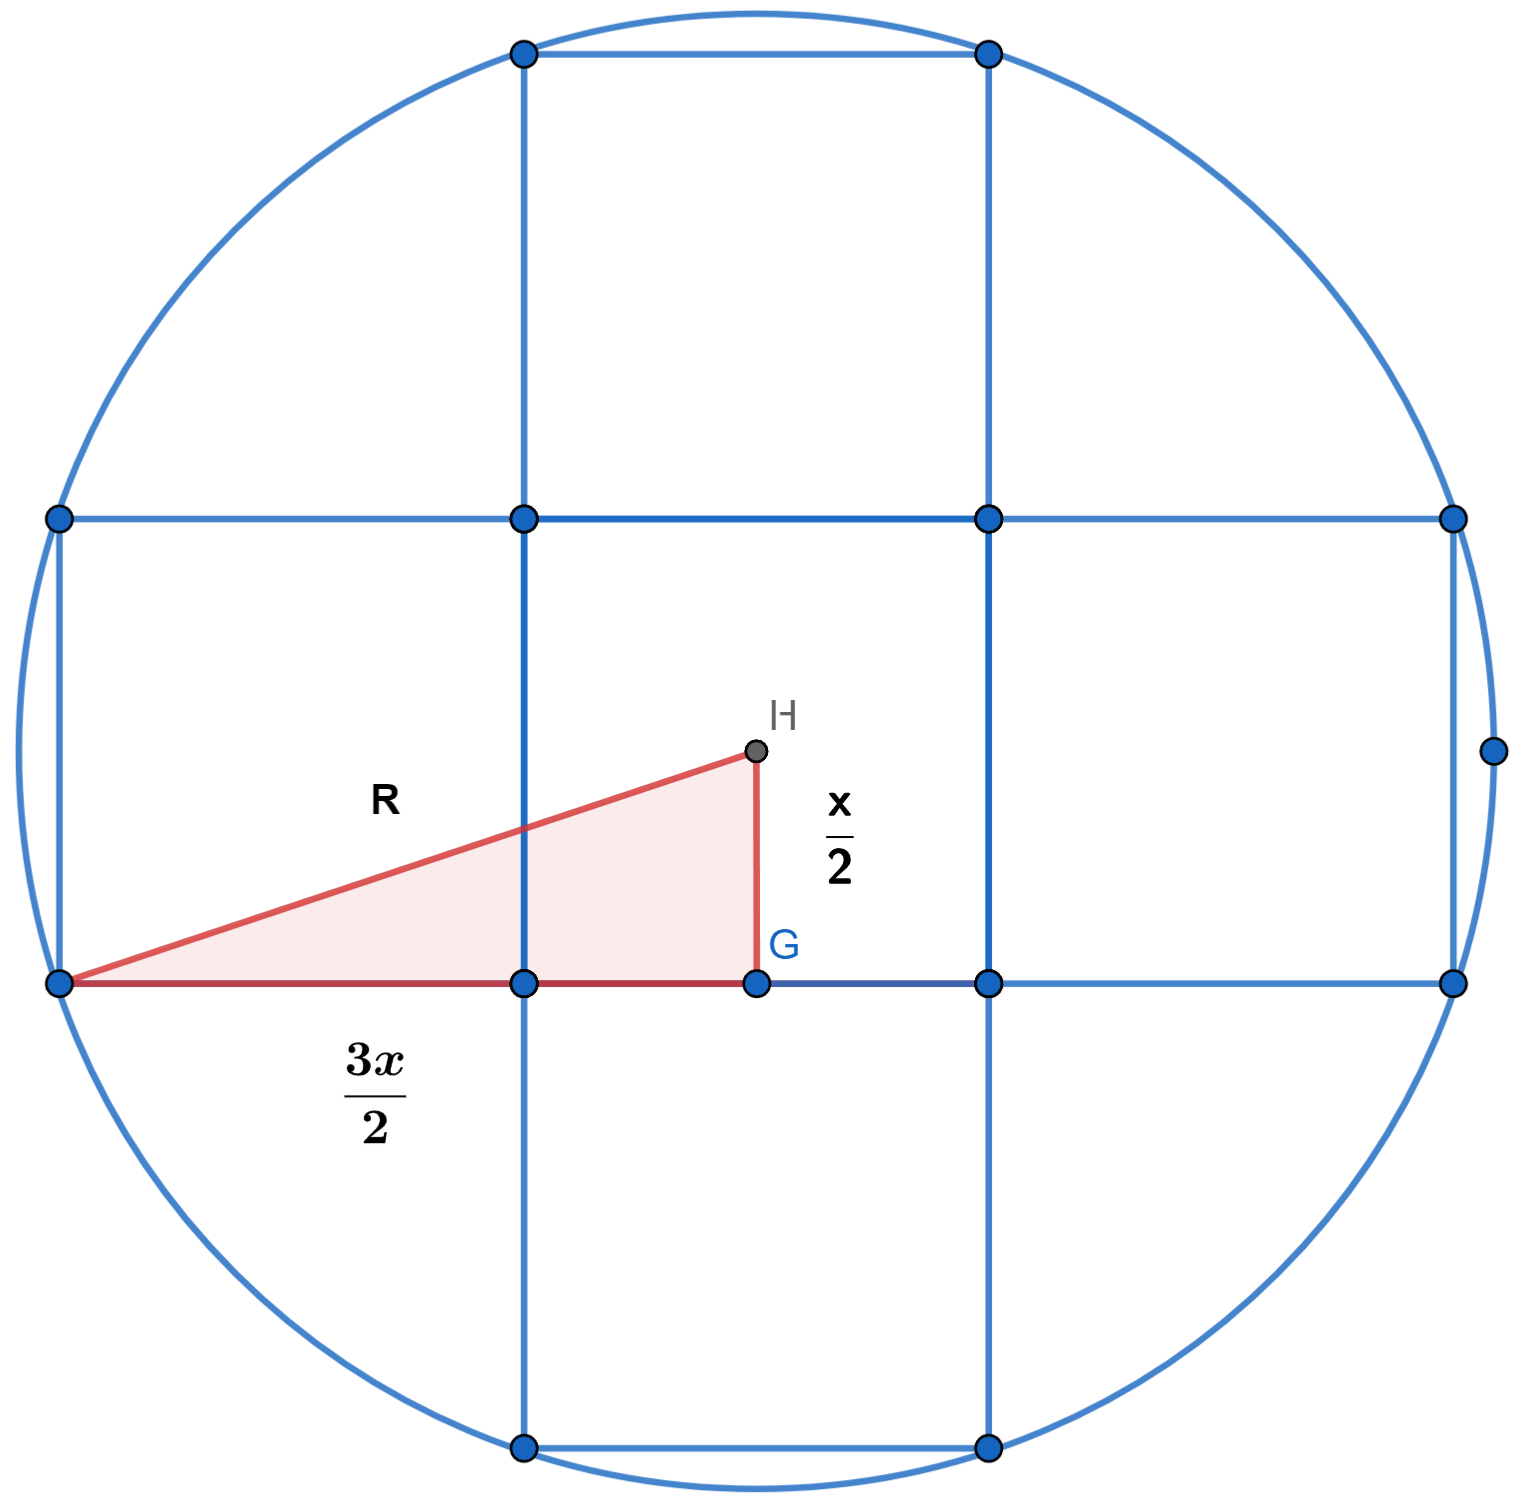
\includegraphics[width=0.5\linewidth]{graphics/marker.png}
    \caption{Diagramm zur Berechnung der Markergrösse}
    \label{fig:marker}
\end{figure}

Die Berechnung der Markergrösse \( x \) basiert auf dem Satz des Pythagoras und kann durch die folgende Funktion beschrieben werden:

\[
f(R) = 2R \cdot \frac{\sqrt{10}}{10}
\]

Für den vom Kunden vorgegebenen Radius von \( R = 10 \, \mathrm{cm} \) ergibt sich:

\[
f(10) = 2 \cdot 10 \cdot \frac{\sqrt{10}}{10} = 2 \cdot \sqrt{10}
\]

Diese Formel liefert eine direkte Methode, die Markergrösse an unterschiedliche Anforderungen anzupassen und dabei eine hohe Präzision in der Berechnung zu gewährleisten.


\subsubsection{Mittelpunkt-Berechnung der Marker Anordnung}
\label{sec:middlePoint}

Um von den 3D Koordinaten der Markern zu den 3D Koordinaten vom Anschlagspunkt zu kommen, muss eine Translation 
gemacht werden. Da die Berechnung zum Mittelpunkt auch mit nur einem Marker funktionieren muss, wird von jede 
Marker-Koordinaten in die Mitte des Keuz-Musters translatiert. Die Anordung der Marker und die damit zusammenhängende 
Marker-ID bestimmt welche Translation durchgeführt werden muss. Marker mit der ID 0 und 4 werden um + l und Marker 
mit ID 2 und 6 um -l in der X-Achse translatiert. Marker mit der ID 1 und 5 werden um -l und Marker mit ID 3 und 7 um +l
in der Y-Achse translatiert. Falls mehrere Marker erkannt werden, wird der Mittelwert aller neuen Punkten genommen.

\begin{figure}[H]
    \centering
    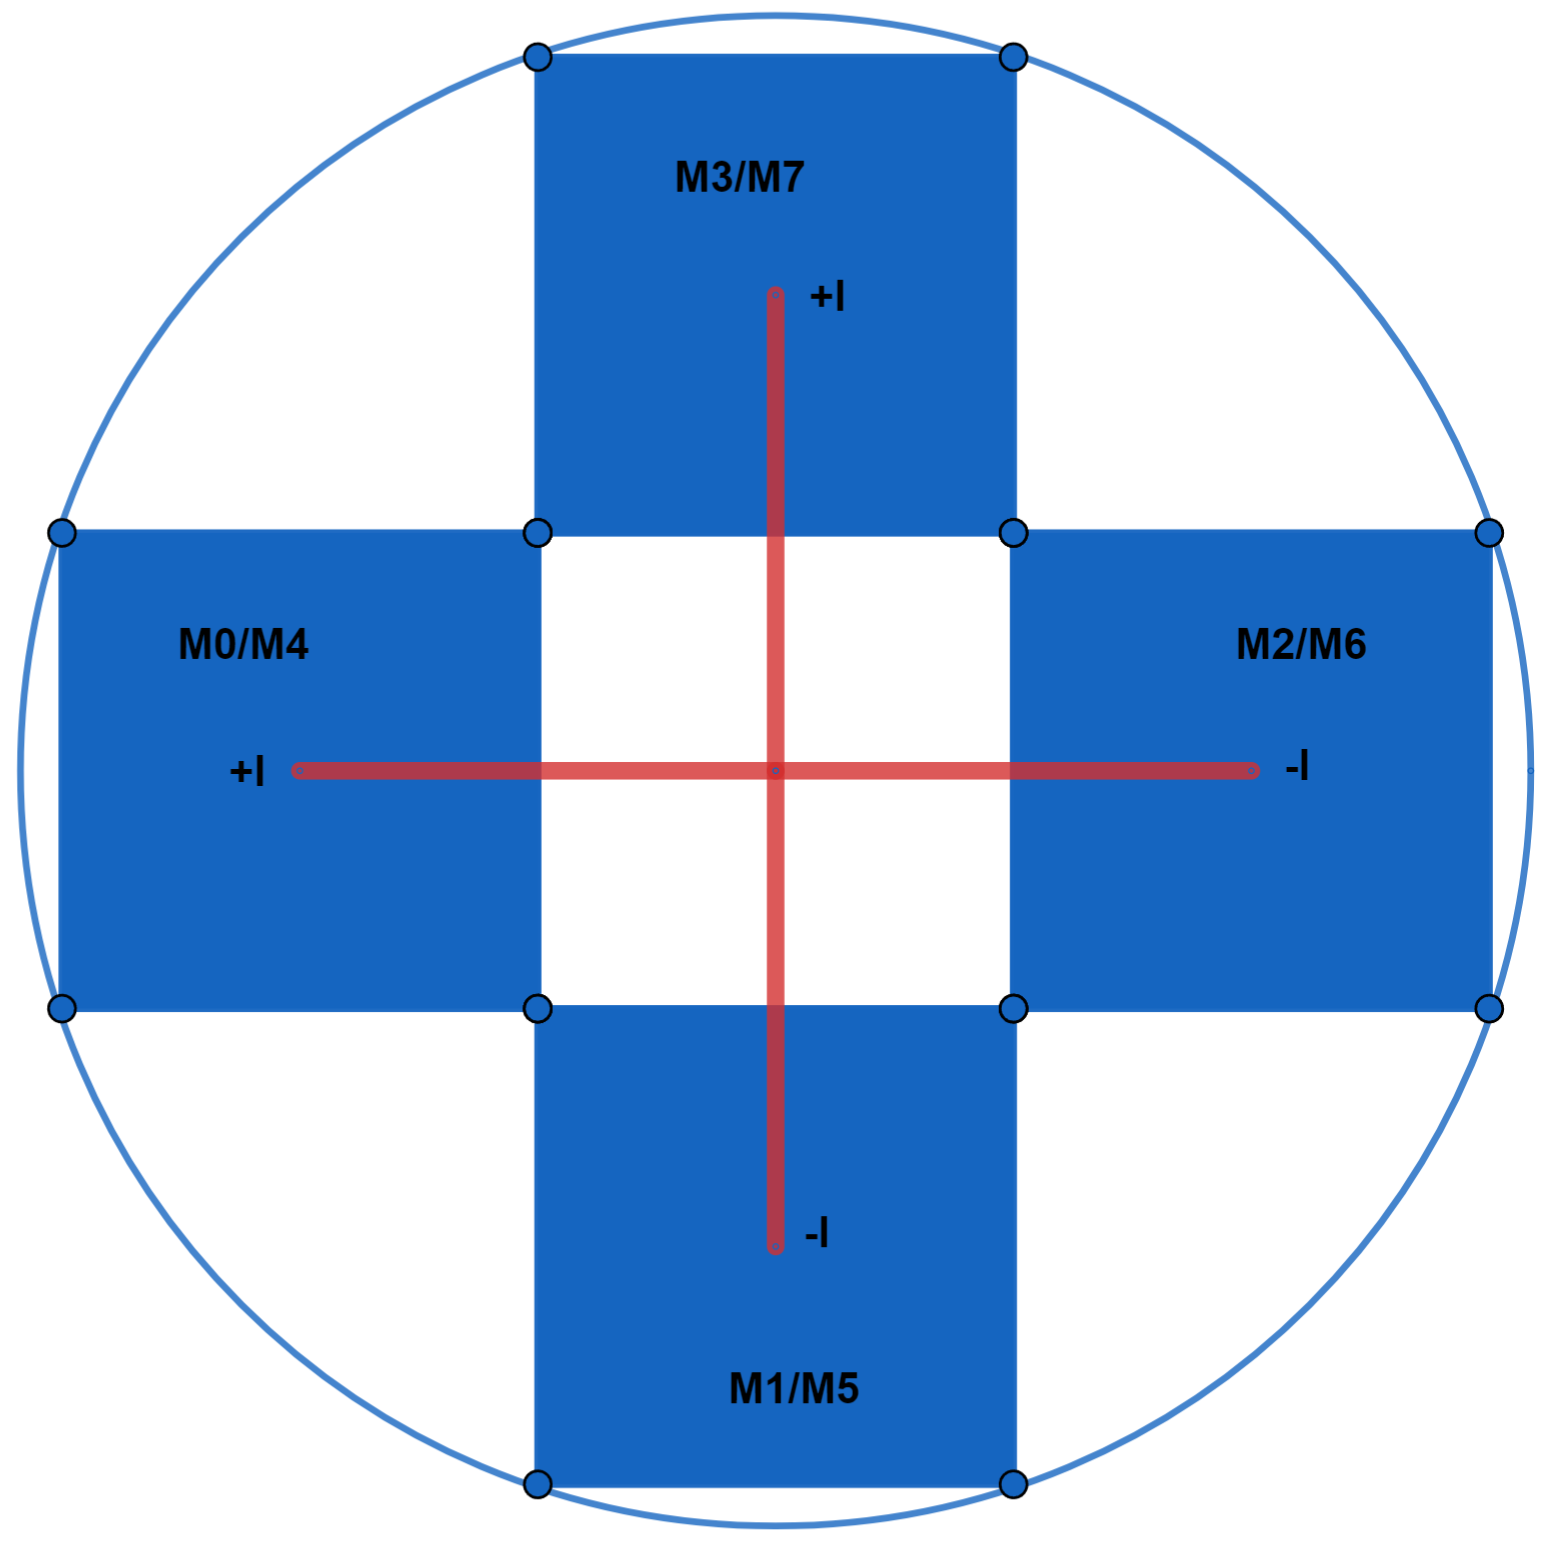
\includegraphics[width=0.5\linewidth]{graphics/marker_anordnung.png}
    \caption{Marker Anordnung für Mittelpunkt rechnung}
    \label{fig:marker_anordnung}
\end{figure}


\subsection{Kamera Eigenschaften}

Um die Anforderungen vom\ref{requirements} zu erfüllen braucht das System eine Kamera, welche sicherstellt dass die Marker genau erkannt werden können.

Dafür ausschlaggebend sind die Markergrösse und eine hohe Bildauflösung\cite{noauthor_designing_2020}. 

Ein weiteres Kriterium für eine genauere Posenschätzung ist die FOV, also Field of View. 
Denn bei höheren FOVs kommt es zu verzerrungen, was dazu resultiert, dass Marker, die weiter von der Bildmitte entfernt sind, keine geraden Linien haben, welches die Posenschätzung ungenauer macht.


\subsubsection{Kamera horizontale Bildwinkel}

Die Kamera sollte von der Mindesthöhe, also 75cm, beide Anschlagspunkte sehen können.

\begin{figure}[H]
    \centering
    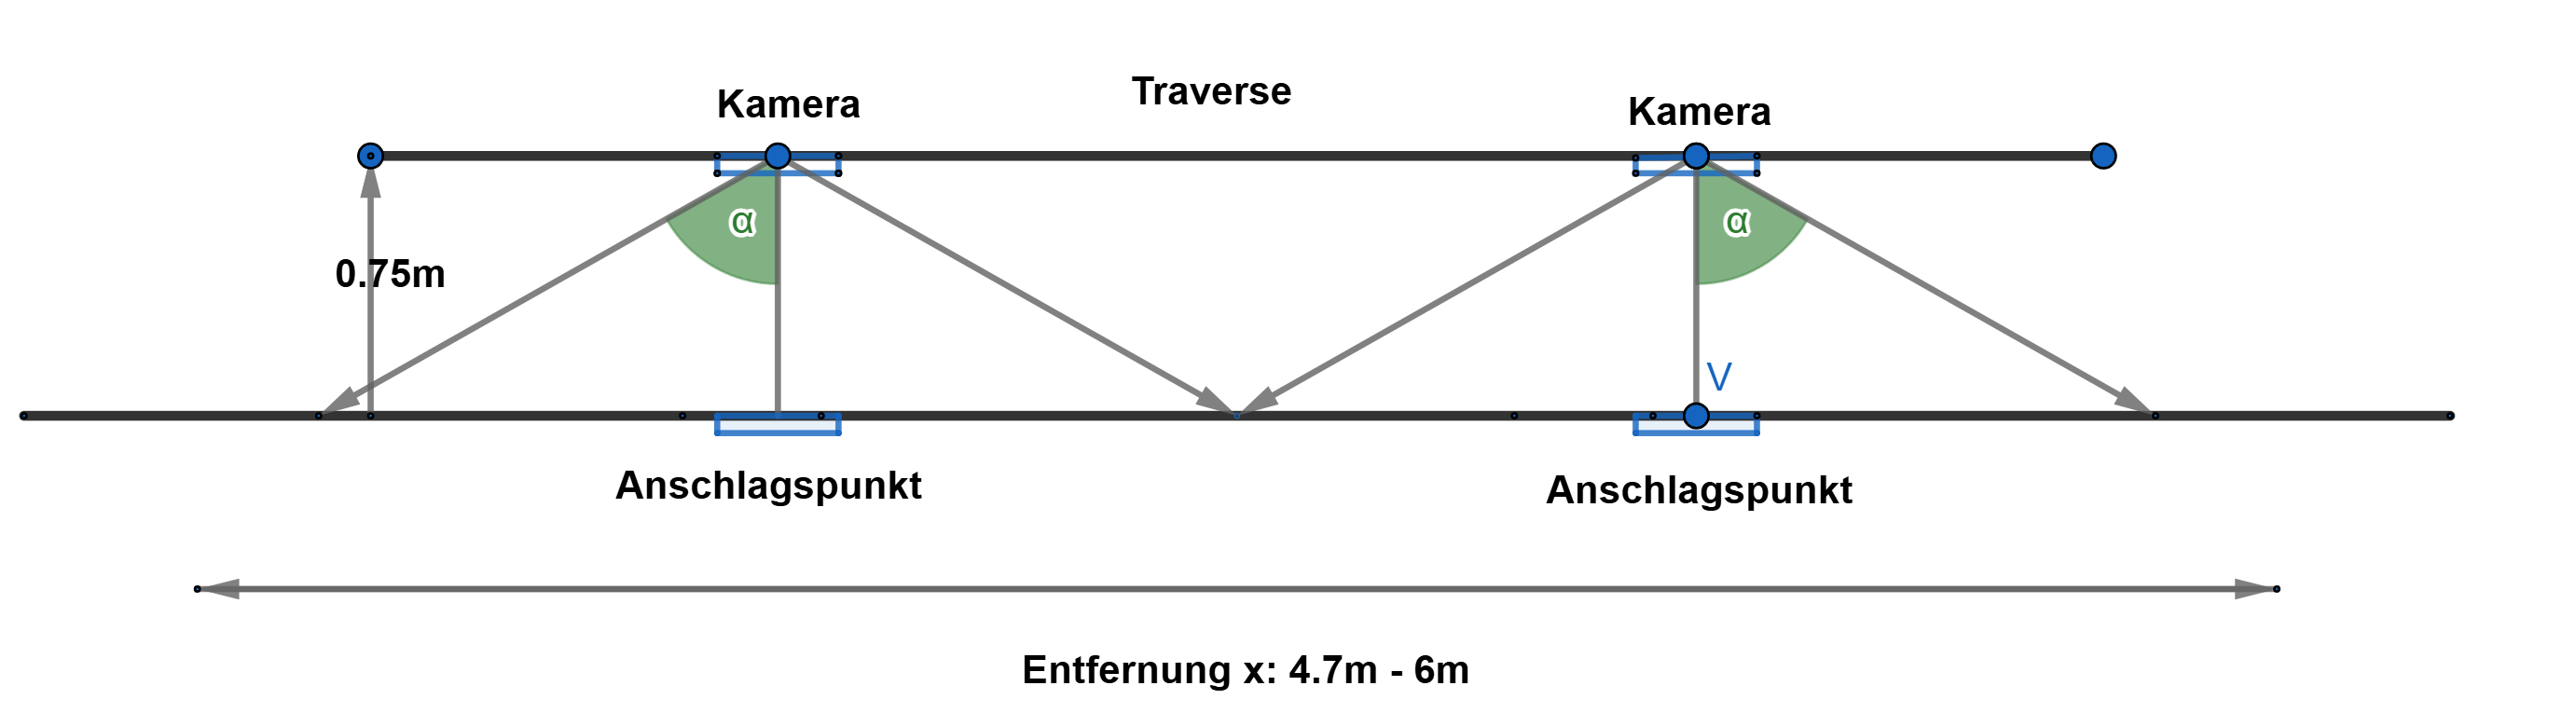
\includegraphics[width=0.5\textwidth]{graphics/KameraFOV.png}\hfill%
    \caption{Kameras decken die Last komplett ab}
    \label{fig:FOV}
\end{figure}

Um einen grossen horizontalen BildWinkel zu vermeiden, wird wie in der Abbildung\ref{fig:FOV} zwei Kameras verwendet. 
Beide Kameras sollten für je ein Anschlagspunkt verantwortlich sein und so im ideal Fall, wenn die Traverse direkt über der Last ist, mindestens von der Mitte der Last bis zum Anschlagspunkt reichen.
Beide Kameras sind dann 117.5cm von der Traversen Mitte entfernt.

Für die Berechnung des horizontalen Bildwinkels werden folgende Variablen benutzt:

Mindesthöhe = h = 75cm\\
Halb-Distanz Mitte-Anschlagspunkt = d = 117.5cm\\

Damit kann man den Bildwinkel \(\alpha\) berechnen welches beide Kameras benutzen müssen:

\begin{equation}
    \alpha = 2*\arctan\frac{d}{h} = 2*\arctan\frac{117.5}{75} = 114.9\degree
    \label{eq:FOV}
\end{equation}


\subsubsection{Kamera Bildauflösung}
Um festzustellen welche Bildauflösung optimal ist, muss die Genauigkeit der Positionierung berechnet werden.

Damit die Genauigkeit der Positionierung berechnet werden kann, muss man erst bestimmen auf wie viele Pixel genau die Lokalisierung ist.

Diese Pixel-Genauigkeit ist variabel, da mit mit Eckenpunkt-Verfeinerungs Methoden SubPixel-Genauigkeiten erreicht werden können.
Diese Methoden sind Zeitaufwändig, da die Iterativ sind, aber erlauben eine bessere Genauigkeit, welches die Posenschätzung verbessert.

Da dass Konzept in Echtzeit funktionieren sollte, wird für die Berechnung der Bildauflösung keine Eckenpunkt-Verfeinerungs Methoden benutzt und ist somit:

Pixel-Genauigkeit = q = 1px\\

Danach muss die Pixelgrösse \(g cm/p\), also die Grösse eines Bildpixels in der Realität, berechnet werden.

\begin{equation}
g = \frac{2*h*\tan\frac{\alpha}{2}}{r} = \frac{2*100*\tan\frac{57.45\degree}{2}}{r} = \frac{313.33cm}{r}
\label{eq:PixelReal}
\end{equation}

In der Formel \ref{eq:PixelReal} wird das horizontale Sichtfeld durch die horizontale Bildauflösung geteilt um so die Grösse jeden Pixels zu erhalten.
Das horizontale Sichtfeld wird mit dem Tangents des Halbwinkel berechnet, welches zusammen mit der Höhe von einem Meter multipliziert wird.
Da dies nur die halbe Sichtweite ist, wird diese verdoppelt um den ganzen horizontalen Sichtfeld zu erhalten.

Mit \(p\) und \(g\) kann die Genauigkeit der Positionierung pro Meter \(t\)  berechnet werden.

\begin{equation}
t = g * q
\label{eq:precision}
\end{equation}

Wenn man jetzt diese Formeln einsetzt für verschiedene Bildauflösungen.

\begin{center}
    \begin{tabular}{ c c}
    \label{tab:resolutions}
     Bildauflösung & Genauigkeit pro Meter\\ 
     \hline
     1920x1080 & 0.163cm \\  
     3840x2160 & 0.082cm \\
     4096x2160 & 0.076cm \\ 
\end{tabular}
\end{center}

Wie die Tabelle zeigt, nimmt die Genauigkeit zu je grösser Die Bildauflösung wird. 
Natürlich sind das Ideal-Werte, da Noise der Kamera und andere externen Bedingungen nicht beachtet wurden. 

\subsection{Evaluation Konzepte}
Um die Lokalisierung durch Machine-Learning durchzuführen braucht es genügend gelabelte Bilder um ein Modell zu trainieren, da kein vortrainiertes Modell vorhanden ist. Das auftreiben und labeln von diesen Bildern würde Zeit und Kosten brauchen. Die Kunden bestätigten das Marker an der Last angebracht werden können und dass sichergestellt werden kann dass diese den gleichen Abstand zueinander haben, weshalb das zweite Konzept ausgewählt wurde.
